\def\SangerLoc{../../Presentations/SangerResource}
\documentclass[]{SangerLibrary/sanger-present}
\usepackage{JML}
\usetikzlibrary{decorations.pathreplacing,calligraphy}
\graphicspath{{Images/}}

\usepackage{fp}
\usepackage{pgfplots}
\usepackage{siunitx}
% \usepackage[usedvipsnames]{xcolor}

\title{\LARGE First Principles of ML\\ {\footnotesize A Peek Inside the 'Black Box' of Machine Learning}}
\author{\large Jack Fraser-Govil}
\institute{The Wellcome Sanger Institute, Hinxton, UK}
\date{\small 15th October 2024}



\renewcommand\vec[1]{\boldsymbol{\mathbf{#1}}}
\begin{document}

	\begin{frame}[fragile]{Today's Resources}
		
		{\large 
		\textbf{Access the Notebook:} 
		\begin{itemize}
			\item Local Clone (\textbf{Recommended}) \verb|git clone https://github.com/wtsi-hpag/xAIWorkshop|
			\item Online Hosting (\textbf{Slow}) Visit \verb|https://githubtocolab.com/wtsi-hpag/xAIWorkshop|
		\end{itemize}
	
		\vspace{1cm}

		\textbf{Interactive Questions} 
		
		(Keep open in a browser tab!)

		\begin{center}
			Join \verb|menti.com| with code \verb|2834 2684|
		\end{center}
		}
	\end{frame}

	\maketitlepage

	{\setbeamercolor{background canvas}{bg=black}
	
	\definecolor{computer}{RGB}{102,255,102}
		\nologo{}
		\begin{frame}[fragile]{\color{computer}Seem Familiar?}
			
			{\color{computer}
			\pause\verb|    >> import ml_toolbox|\par\par
			\pause \verb|    >> data,labels = load_my_data()|\par\par
			\pause \verb|    >> model = ml_toolbox.make_model(layers=5,func=sigmoid)|\par\par
			\pause \verb|    >> model.Train(data,labels,epochs=1000)|\par~\par
			\pause\verb@    Epoch 0: 0%|                | [0/1000 10it/s, loss = 10.4]@\par~\par
			% \only<6>\verb@    Epoch x: 10%|x                | [880/1000 10it/s, loss = 0.4]@

			~
			}
		\end{frame}
		\begin{frame}[fragile]{\color{computer}Seem Familiar?}
			
			{\color{computer}
			\verb|    >> import ml_toolbox|\par\par
			\verb|    >> data,labels = load_my_data()|\par\par
			\verb|    >> model = ml_toolbox.make_model(layers=5,func=sigmoid)|\par\par
			\verb|    >> model.Train(data,labels,epochs=1000)|\par~\par
			\verb@    Epoch 100: 10%|xx              | [100/1000 10it/s, loss = 5.5]@\par~\par~
			% \only<6>\verb@    Epoch x: 10%|x                | [880/1000 10it/s, loss = 0.4]@
			}
		\end{frame}
		\begin{frame}[fragile]{\color{computer}Seem Familiar?}
			
			{\color{computer}
			\verb|    >> import ml_toolbox|\par\par
			\verb|    >> data,labels = load_my_data()|\par\par
			\verb|    >> model = ml_toolbox.make_model(layers=5,func=sigmoid)|\par\par
			\verb|    >> model.Train(data,labels,epochs=1000)|\par~\par
			\verb@    Epoch 200: 20%|xxxx            | [200/1000 12it/s, loss = 3.4]@\par~\par~
			% \only<6>\verb@    Epoch x: 10%|x                | [880/1000 10it/s, loss = 0.4]@
			}
		\end{frame}
		\begin{frame}[fragile]{\color{computer}Seem Familiar?}
			
			{\color{computer}
			\verb|    >> import ml_toolbox|\par\par
			\verb|    >> data,labels = load_my_data()|\par\par
			\verb|    >> model = ml_toolbox.make_model(layers=5,func=sigmoid)|\par\par
			\verb|    >> model.Train(data,labels,epochs=1000)|\par~\par
			\verb@    Epoch 300: 30%|xxxxxx          | [300/1000 9it/s, loss = 3.1]@\par~\par~
			% \only<6>\verb@    Epoch x: 10%|x                | [880/1000 10it/s, loss = 0.4]@
			}
		\end{frame}
		\begin{frame}[fragile]{\color{computer}Seem Familiar?}
			
			{\color{computer}
			\verb|    >> import ml_toolbox|\par\par
			\verb|    >> data,labels = load_my_data()|\par\par
			\verb|    >> model = ml_toolbox.make_model(layers=5,func=sigmoid)|\par\par
			\verb|    >> model.Train(data,labels,epochs=1000)|\par~\par
			\verb@    Epoch 400: 40%|xxxxxx          | [400/1000 16it/s, loss = 2.9]@\par~\par~
			% \only<6>\verb@    Epoch x: 10%|x                | [880/1000 10it/s, loss = 0.4]@
			}
		\end{frame}
		\begin{frame}[fragile]{\color{computer}Seem Familiar?}
			
			{\color{computer}
			\verb|    >> import ml_toolbox|\par\par
			\verb|    >> data,labels = load_my_data()|\par\par
			\verb|    >> model = ml_toolbox.make_model(layers=5,func=sigmoid)|\par\par
			\verb|    >> model.Train(data,labels,epochs=1000)|\par~\par
			\verb@    Epoch 500: 50%|xxxxxxxxx       | [500/1000 12it/s, loss = 1.4]@\par~\par~
			% \only<6>\verb@    Epoch x: 10%|x                | [880/1000 10it/s, loss = 0.4]@
			}
		\end{frame}
		\begin{frame}[fragile]{\color{computer}Seem Familiar?}
			
			{\color{computer}
			\verb|    >> import ml_toolbox|\par\par
			\verb|    >> data,labels = load_my_data()|\par\par
			\verb|    >> model = ml_toolbox.make_model(layers=5,func=sigmoid)|\par\par
			\verb|    >> model.Train(data,labels,epochs=1000)|\par~\par
			\verb@    Epoch 700: 70%|xxxxxxxxxxxx    | [700/1000 5it/s, loss = 1.39]@\par~\par~
			% \only<6>\verb@    Epoch x: 10%|x                | [880/1000 10it/s, loss = 0.4]@
			}
		\end{frame}
		\begin{frame}[fragile]{\color{computer}Seem Familiar?}
			
			{\color{computer}
			\verb|    >> import ml_toolbox|\par\par
			\verb|    >> data,labels = load_my_data()|\par\par
			\verb|    >> model = ml_toolbox.make_model(layers=5,func=sigmoid)|\par\par
			\verb|    >> model.Train(data,labels,epochs=1000)|\par~\par
			\verb@    Epoch 900: 90%|xxxxxxxxxxxxxxx | [900/1000 8it/s, loss = 1.385]@\par~\par~
			% \only<6>\verb@    Epoch x: 10%|x                | [880/1000 10it/s, loss = 0.4]@
			}
		\end{frame}
		\begin{frame}[fragile]{\color{computer}Seem Familiar?}
			
			{\color{computer}
			\verb|    >> import ml_toolbox|\par\par
			\verb|    >> data,labels = load_my_data()|\par\par
			\verb|    >> model = ml_toolbox.make_model(layers=5,func=sigmoid)|\par\par
			\verb|    >> model.Train(data,labels,epochs=1000)|\par~\par
			\verb@    Epoch 1000: 100%|xxxxxxxxxxxxxxxx| [final loss = 1.382]@\par~\par
			% \only<6>\verb@    Epoch x: 10%|x                | [880/1000 10it/s, loss = 0.4]@
			\pause\verb|    >> model.Test()|
			}
			
		\end{frame}
		
	}
	% \beginn{frame}

	\begin{frame}{Today's Agenda}
		The aim for today is:

		\begin{itemize}
			\pitem Classic Perceptron
			\pitem Feedforward Networks
			\pitem Non-Linearity
			\pitem Optimisation \& Backpropagation
		\end{itemize}

		\pause As we progress you will slowly build up your own ML toolkit, built entirely from scratch! 

	\end{frame}

	% \begin{frame}{}
	\newcounter{custompart}
	\setcounter{custompart}{0}
	\newcommand\partFrame[1]
	{
		\stepcounter{custompart}
		\begin{frame}{}
			\begin{center}
				\Wellcome \huge Part \thecustompart

				#1
			\end{center}
		\end{frame}
	}
	% \end{frame}
	
	\begin{frame}{A Warning}
		
		\begin{center}
			{\Large There will be equations.}
			
			{\pause \Large You will need to know what they mean!}

			{\pause \it Please, please, please, ask if you want clarification on the underlying mathematics and theory! That's why you're here today!} 
		\end{center}
	\end{frame}


	\partFrame{The Perceptron}
	
\def\cuteB{-3}
\def\cuteWA{0}
\def\cuteWB{1}
\def\learn{0.01}
\newcommand\cute[5]
	{
		\def\cuteLabel{#5}
		\def\labelText{Not Cute}
		\ifnum\cuteLabel=1
			\def\labelText{Cute}
		\fi
		\node at ({#1},{#2}) {\includegraphics[width=2cm,height=2cm,keepaspectratio=true]{#3}};
		
		% \node at ({#1},{#2}) {#4 \highlight{}};
		\def\test{#4}
		\def\comp{\highlight}




		%%%PERCEPTRON IMPLEMENTED WITHIN IMAGE PLACEMENT
		\ifnum\test=\comp

			\FPeval{dot}{(\a) + (#1*(\b)) + (#2*(\c))}
			\def\cuteGuess{0}
			\pgfmathparse{\dot<0}

			%COMPUTE ASSIGNED VALUE
			\ifnum\pgfmathresult=0
				\def\cuteGuess{1}
			\fi
			\def\guessText{Not Cute}
			\if\cuteGuess1
				\def\guessText{Cute}
			\fi
			
			%DRAW COLOUR
			\def\highcolour{\wrongcolour}
			\ifnum\cuteGuess=\cuteLabel
				\def\highcolour{\rightcolour}
			\else

				%%%UPDATE WEIGHTS IF GUESSED WRONG
				\xdef\updated{1}
				\FPeval{bup}{(\cuteB) + ((\cuteLabel)-(\cuteGuess))*(\learn)}
				\FPeval{waup}{(\cuteWA) + ((\cuteLabel)-(\cuteGuess))*(\learn)*(#1)}
				\FPeval{wbup}{(\cuteWB) + ((\cuteLabel)-(\cuteGuess))*(\learn)*(#2)}
				\xdef\cuteB{\bup}
				\xdef\cuteWA{\waup}
				\xdef\cuteWB{\wbup}
			\fi
			\fill[\highcolour,opacity=0.2] ({#1},{#2}) circle (1.3);
			% \node[red] at ({#1},{#2}) {\a +#1* \b + #2 * \c = \dot};
			
			\node at ({#1},{#2+1.1}) {\tiny Labelled: \labelText, Guess \guessText};
		\else
			% \node at ({#1},{#2-1.1}) {\tiny \labelText};
		\fi
		
	}
% \setbeamercolor{background canvas}{bg=SangerLight}
% \logo{\SangerLogoBlack}
\def\highlight{0}
\def\rightcolour{green!70!black}
\def\wrongcolour{red!70!black}
\def\highcolour{\rightcolour}
\newcommand\animals{
	\cute{0.7}{3.5}{mouse}{1}{1}
	\cute{2}{6}{rabbit}{2}{1}
	\cute{6}{5.7}{dog}{3}{1}
	\cute{4}{5.8}{cat}{4}{1}
	\cute{9}{5.5}{lion}{5}{0}
	\cute{10}{1}{whale}{6}{0}
	\cute{7}{2.7}{warthog}{7}{0}
	\cute{1.7}{1}{molerat}{8}{0}
	\cute{4}{2}{ayeaye}{9}{0}
	\cute{0.1}{0.1}{ant}{10}{0}
}

\newcommand\confusing{
	\cute{2}{6}{rabbit}{1}{1}
	\cute{9}{5.5}{lion}{2}{0}
	\cute{10}{1}{whale}{3}{1}
	\cute{0.1}{0.1}{ant}{4}{0}
}
	\begin{frame}{Basic Decision Making: Defining Cuteness}

		
		\begin{center}
			\def\w{8}
			\begin{tikzpicture}

				\animals
				\draw[->] (0,0)--node[below]{Size} (10,0);
				\draw[->] (0,0)--node[left]{Fur} (0,6);
				\pause \draw[dashed] (0,1)--node[above,rotate=30] {\textbf{Cute}} node[below,rotate=30] {\textbf{Not Cute}} (8,6);

			\end{tikzpicture}
		\end{center}

	\end{frame}

	
	\begin{frame}{Splitting The Plane}
		In order to split the plane into two parts, we merely need to define a \textit{line}. 
		
		\begin{center}
			\begin{tikzpicture}
			
				\begin{axis}[xmin = 0, xmax = 10, ymin = 0, ymax = 6, ylabel={Fur}, xlabel ={Size},x post scale = 1]
					\addplot[domain = 0:10, samples = 200,blue]{5/8*x+1};
						\end{axis}
			
			\end{tikzpicture}
			\end{center}
	\end{frame}

	\begin{frame}{Splitting the plane}
		\pause \textbf{Question: } If we have $N$ dimensions ($N=2$), how many parameters do we need to define a line?
		
		\vspace{2cm}
		
		\pause \textbf{Answer: } The answer is $N$ - in 2 dimensions, this is friendly $y = mx + c \to (m,c)$

		% \pause \textbf{Question: } Why then do we need $N+1$ dimensions?
	\end{frame}

	\begin{frame}{The Perceptron}
		% We need 3 parameters to define a \textbf{directional line}. 
		
		The Perceptron classifier algorithm is:
		
		\only<1>{\begin{equation}
			P(\vec{x}) = \begin{cases} 1 & \text{if } b + \vec{w} \cdot \vec{x}\footnote{The dot/inner product is covered in Section 3.1 in the notes} > 0 \\ 0 &\text{else} 
		\end{cases}
		\end{equation}}

		\only<2,3>{\begin{equation}
			P(\vec{x}) = \begin{cases} 1 & \text{if } \tilde{\vec{x}} \cdot \vec{w}\footnote{The dot/inner product is covered in Section 3.1 in the notes} > 0 \\ 0 &\text{else} 
		\end{cases}
		\end{equation}}

		\pause Where 
		$$\tilde{\vec{x}} = \begin{pmatrix}
			1 \\ \vec{x}
		\end{pmatrix}$$
		\pause $\vec{w}$ are the \textbf{weights}. 

		
	\end{frame}

	\begin{frame}{The Perceptron: Dimensions}
		\textbf{Question:} What is the dimensionality of the Perceptron? Does this conflict with our earlier statements?

		\vspace{1cm}

		\pause \textbf{Hint:} It has nothing to do with the `bias'!

		\vspace{1cm}

		\pause \textbf{Answer:} We need $N+1$ dimensions. $N$ dimensions define a line - but need an additional dimension to add \textit{directionality}
	\end{frame}

	\begin{frame}{The Perceptron: Dimensions}
		
		\only<1>{\begin{center}
			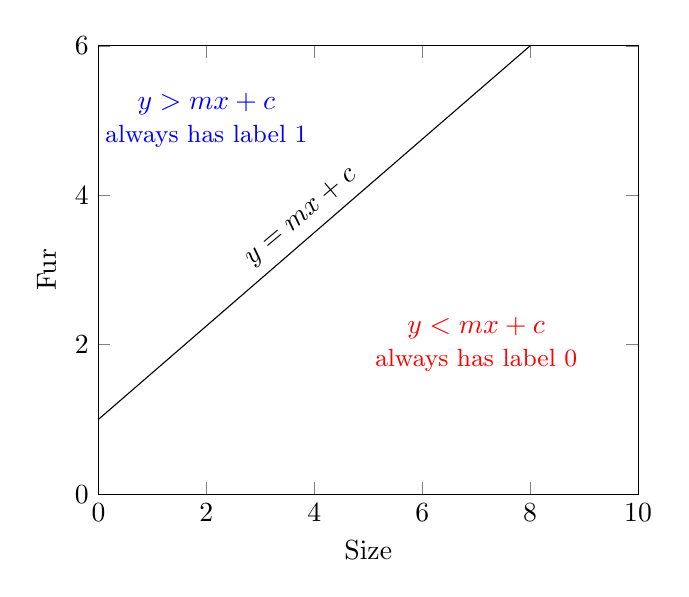
\begin{tikzpicture}
			
				\begin{axis}[xmin = 0, xmax = 10, ymin = 0, ymax = 6, ylabel={Fur}, xlabel ={Size},x post scale = 1]
					\addplot[domain = 0:8, samples = 200,black]{5/8*x+1} node[midway,above,rotate=40] {$y= mx + c$};

					\node[rotate=0,blue] at (axis cs: 2,5) {\parbox[t]{18cm}{\centering $y> mx + c$ \\ {\small always has label 1}}};

					\node[red] at (axis cs: 7,2) {\parbox[t]{18cm}{\centering $y< mx + c$ \\ {\small always has label 0}}};
						\end{axis}
			
			\end{tikzpicture}
			\end{center}}

			\only<2>{\begin{center}
				\begin{tikzpicture}
				
					\begin{axis}[xmin = 0, xmax = 10, ymin = 0, ymax = 6, ylabel={Fur}, xlabel ={Size},x post scale = 1]
						\addplot[domain = 0:8, samples = 200,black]{5/8*x+1} node[midway,below,rotate=40] {$|v|\begin{bmatrix} -c  \\ -m  \\ +1 \end{bmatrix} \cdot \begin{bmatrix} 1 \\ x \\ y \end{bmatrix} > 0$};
	
						\node[rotate=0,blue] at (axis cs: 2,5) {\parbox[t]{18cm}{\centering $y> mx + c$ \\ {\small has label 1}}};
	
						\node[red] at (axis cs: 7,1) {\parbox[t]{18cm}{\centering $y< mx + c$ \\ {\small has label 0}}};
							\end{axis}
				
				\end{tikzpicture}
				\end{center}}


				\only<3>{\begin{center}
					\begin{tikzpicture}
					
						\begin{axis}[xmin = 0, xmax = 10, ymin = 0, ymax = 6, ylabel={Fur}, xlabel ={Size},x post scale = 1]
							\addplot[domain = 0:8, samples = 200,black]{5/8*x+1} node[midway,below,rotate=40] {$|v|\begin{bmatrix} -c  \\ -m  \\ -1 \end{bmatrix} \cdot \begin{bmatrix} 1 \\ x \\ y \end{bmatrix} > 0$};
		
							\node[rotate=0,red] at (axis cs: 2,5) {\parbox[t]{18cm}{\centering $y> mx + c$ \\ {\small has label 0}}};
		
							\node[blue] at (axis cs: 7,1) {\parbox[t]{18cm}{\centering $y< mx + c$ \\ {\small has label 1}}};
								\end{axis}
					
					\end{tikzpicture}
					\end{center}}
	\end{frame}

	\begin{frame}[fragile]{Exercise 1: Perceptron Classifier}
		% \begin{center}
			\textbf{Task 1: } Write a perceptron classifier for the data in \verb|cuteness.dat|

			\vspace{1cm}

			\textbf{Guidance:} Class structure \& predetermined weights are provided in the notebook. Ignore \verb|Train()| for now

			\vspace{1cm}

			\textbf{Question:}	The provided weights classify only one animal correctly. Which is it?
		% \end{center}
	\end{frame}


	\begin{frame}{Training A Perceptron}
		Training a perceptron is easy. Loop over the data, make a prediction ($P$), compare it to the truth  ($T$) and if it is wrong:

		\pause \begin{equation}
			\vec{w} \to \vec{w} + r \times \left(T - P\right) \tilde{\vec{x}}
		\end{equation}

		\pause This works because it always makes $\vec{w} \cdot \tilde{\vec{x}}$ move closer towards zero (and hence to the tipping point of altering its decision).

	\end{frame}

	\begin{frame}[fragile]{Exercise 2: Train Your Perceptron}

			\textbf{Task 2:} Write the \verb|Train()| method for your Perceptron, then apply to \verb|cuteness| data.

			\vspace{1cm}

			\pause\textbf{Question:}	How long does it take to train to 100\% accuracy?

			\pause Give your answers on \verb|menti.com| with code \verb|2834 2684|
	\end{frame}

	\begin{frame}[fragile]{Exercise 3: The Limits of Linearity}
		
		\textbf{Task 3:} Apply your method to the data in \verb|cuteness_augmented.dat|, which adds the Axolotl, Otter, Capybara, Quokka, Slug, Tasmanian Devil and Giant Panda.

		\textbf{Question:} What has gone wrong? Who are the troublemakers?

		\only<2>{\centering 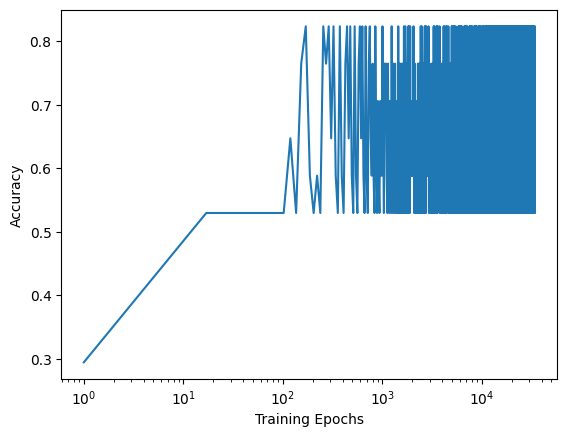
\includegraphics[width=0.8\linewidth,height=0.7\paperheight,keepaspectratio=true]{accuracy_bigStep.png}}

		\only<3>{\centering 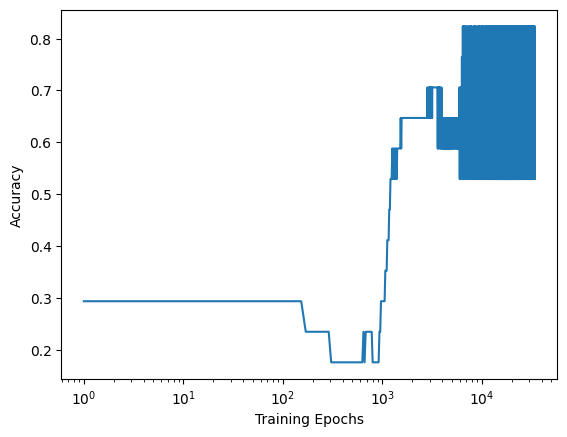
\includegraphics[width=0.8\linewidth,height=0.7\paperheight,keepaspectratio=true]{accuracy_smallStep.png}}
	\end{frame}

	\begin{frame}{The Nonlinear Perceptron}
		Eminently possible to have a non-linear perceptron. 
		
		\pause Pass $\vec{x}$ through a non-linear transform to make it:

		\begin{equation}
			\vec{x}^\prime = \begin{pmatrix}
				1 \\ x \\ y \\ x^2 \\ \sin(x) \\ x^2 \exp(y) \\ \cos(\sin(\exp(\sin(\log(x^2 + 9 xy))))) \\ \vdots \end{pmatrix}
		\end{equation}

	\end{frame}

	\begin{frame}{The Nonlinear Perceptron}
		Here is the results of a perceptron where:

		\setcounter{MaxMatrixCols}{20}
		\begin{equation}
			\vec{x}^\prime(x,y) = \begin{pmatrix}
				1 & x & y & x^2 & xy & y^2 & x^3 & x^2y & xy^2 & y^3 & x^4 & x^3y & x^2y^2 & xy^3 & y^4
			\end{pmatrix}^\intercal
		\end{equation}


		\textit{Bonus Question: Why did I choose this?}

	\end{frame}

	\begin{frame}{The Nonlinear Perceptron}
		

		{\centering 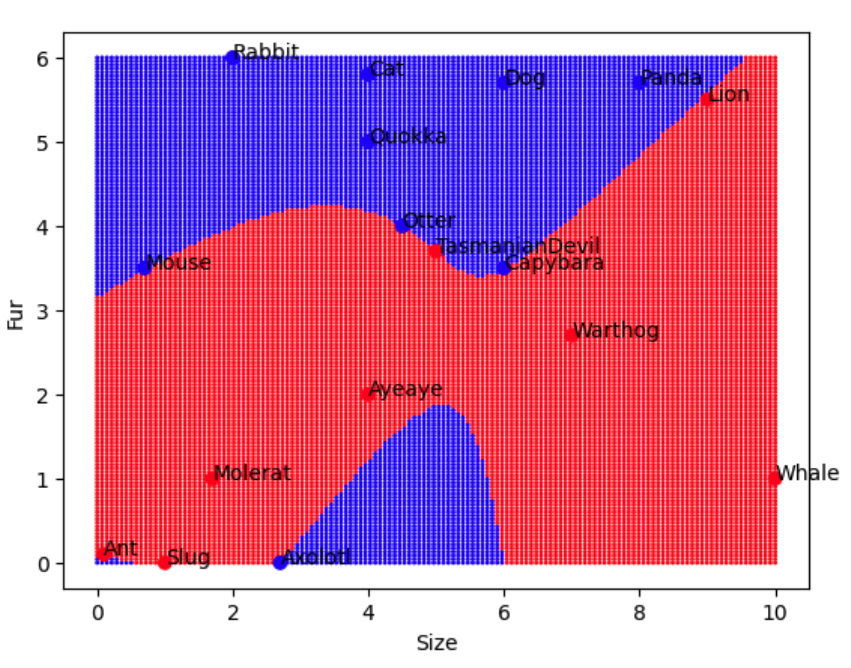
\includegraphics[width=0.8\linewidth,height=0.8\paperheight,keepaspectratio=true]{NonLinear.png}}

	\end{frame}

	\begin{frame}{The Limits of NonLinearity}
		

		\begin{minipage}{0.5\linewidth}
			\textbf{Target}

			{\centering 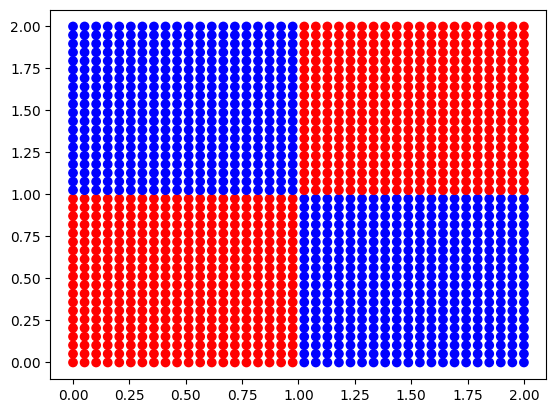
\includegraphics[width=\linewidth,height=0.8\paperheight,keepaspectratio=true]{xor_full.png}}
		\end{minipage}\begin{minipage}{0.5\linewidth}

			\only<2>{\textbf{Reality (1st Order - 3 parameters)}
				
			\centering 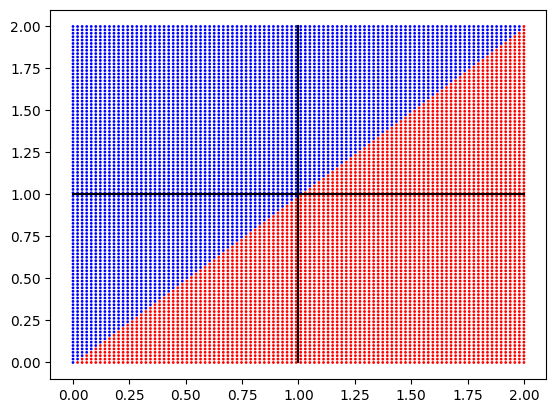
\includegraphics[width=\linewidth,height=0.8\paperheight,keepaspectratio=true]{xor_1.png}}

			\only<3>{\textbf{Reality (2nd Order - 6 parameters)}
				
			\centering 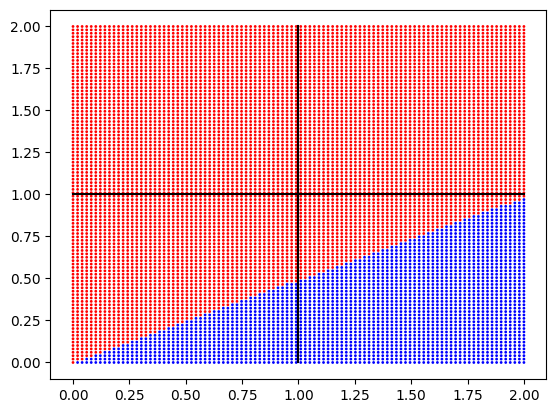
\includegraphics[width=\linewidth,height=0.8\paperheight,keepaspectratio=true]{xor_2.png}}

			\only<4>{\textbf{Reality (3rd Order - 10 parameters)}
				
			\centering 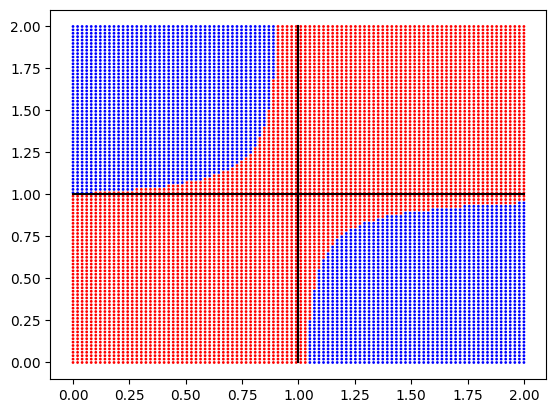
\includegraphics[width=\linewidth,height=0.8\paperheight,keepaspectratio=true]{xor_3.png}}

			\only<5>{\textbf{Reality (4th Order - 15 parameters)}
				
			\centering 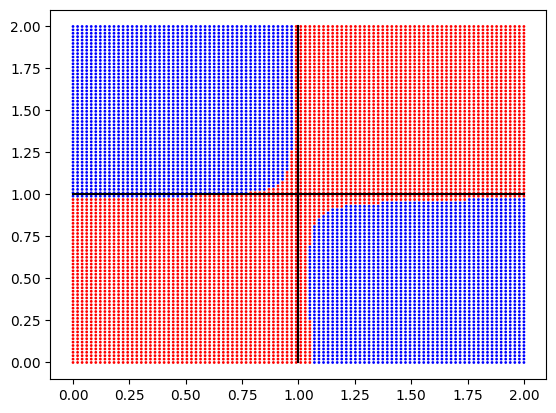
\includegraphics[width=\linewidth,height=0.8\paperheight,keepaspectratio=true]{xor_4.png}}

			\only<6>{\textbf{Reality (5th Order - 21 parameters)}
				
			\centering 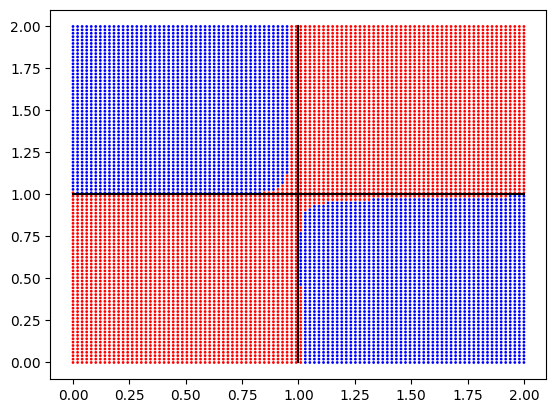
\includegraphics[width=\linewidth,height=0.8\paperheight,keepaspectratio=true]{xor_5.png}}

			\only<7>{\textbf{Reality (5th Order - 21 parameters)}
				
			\centering 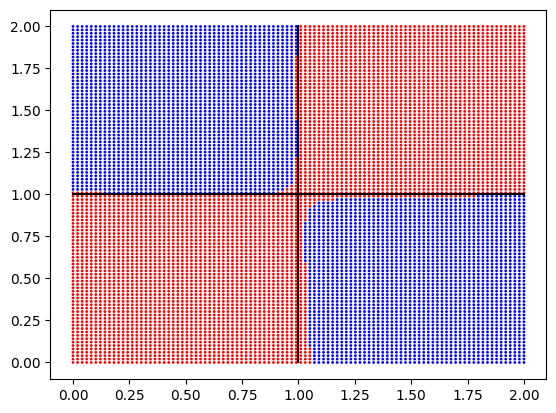
\includegraphics[width=\linewidth,height=0.8\paperheight,keepaspectratio=true]{xor_10.png}}

			\only<8>{\textbf{Reality (20th Order - 231 parameters)}
				
			\centering 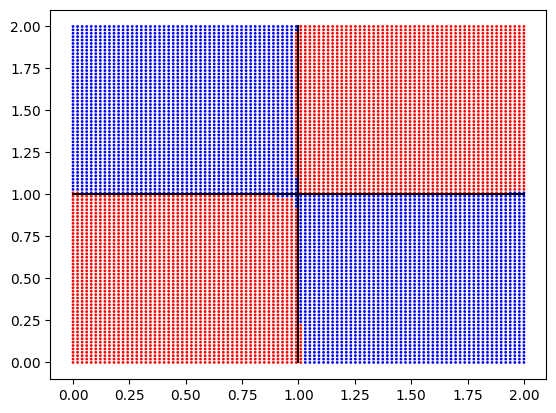
\includegraphics[width=\linewidth,height=0.8\paperheight,keepaspectratio=true]{xor_20.png}}
		\end{minipage}
		

	\end{frame}
	

	\begin{frame}{What do to?}
		\begin{center}
			\pause MORE!
		\end{center}
	\end{frame}

	\newcommand\cec[1]{{\vec{#1}}}
	{

	\nologo
	\begin{frame}{The Multilayered Perceptron}
		% Let's try chaining lots of pecreptrons together.....
		
		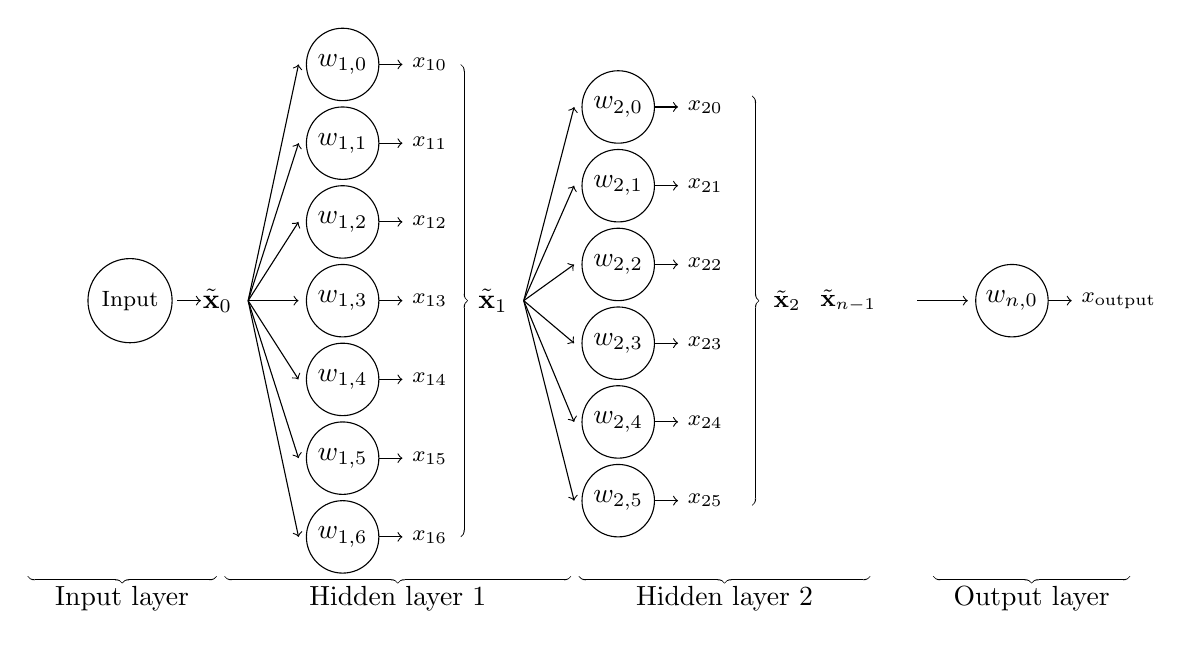
\begin{tikzpicture}
			% \draw (0,0) circle (0.4);
			\pause\node[draw,circle] at (0.3,0) {\footnotesize Input};
			\draw[->] (0.9,0)--(1.2,0);
			\def\baseheight{-3.5}
			\draw [decorate, decoration = {calligraphic brace}] (1.4,\baseheight) --node[below]{Input layer}  (-1,\baseheight);
			\node[anchor=west] at (1.1,0) {$\tilde{\vec{x}}_0$};

			\pause
			
			
			% \draw [decorate, decoration = {calligraphic brace}] (1.3,1.2) --  (1.3,-1.2);
			
			\foreach \i[count=\j from 0] in {3,2,...,-3}
			{
				\def\r{0.46}
				\def\y{\i}
				\def\x{3}
				\draw[->] (1.8,0)--({\x-\r-0.1},\y);
				\draw (\x,{\y}) circle ({\r});
				\node at (\x,{\y}) { $\cec{w}_{1,\j}$};
				\draw [->] ({\x+\r},{\y})--({\x+\r+0.3},{\y});
				\def\xx{\x+\r+0.3}
				% \draw[fill=white] ({\x-\r},{\y-\r})--({\x+\r},{\y-\r})--({\x+\r},{\y+\r})--({\x-\r},{\y+\r})--cycle;
				\node[anchor=west] at (\xx,{\y}) {\fontsize{8}{0}\selectfont$x_{1\j}$};%\phi_{1}^{\j}(y_{1}^{\j})$};
			}
			\pause\draw [decorate, decoration = {calligraphic brace}] (4.5,3) --  (4.5,-3);
			\node[anchor=west] at (4.6,0) {$\tilde{\vec{x}}_1$};
			\pause\draw [decorate, decoration = {calligraphic brace}] (5.9,\baseheight) --node[below]{Hidden layer 1}  (1.5,\baseheight);
			
			\pause

			\foreach \i[count=\j from 0] in {2,1,0,-1,-2,-3}
			{
				\def\r{0.46}
				\def\y{\i+\r}
				\def\x{6.5}
				\draw[->] (5.3,0)--({\x-\r-0.1},\y);
				\draw (\x,{\y}) circle ({\r});
				\node at (\x,{\y}) { $\cec{w}_{2,\j}$};
				\draw [->] ({\x+\r},{\y})--({\x+\r+0.3},{\y});
				\def\xx{\x+\r+0.3}
				% \draw[fill=white] ({\x-\r},{\y-\r})--({\x+\r},{\y-\r})--({\x+\r},{\y+\r})--({\x-\r},{\y+\r})--cycle;
				\node[anchor=west] at (\xx,{\y}) {\fontsize{8}{0}\selectfont$x_{2\j}$};%\phi_{2}^{\j}(y_{2}^{\j})$};
			}
			\draw [decorate, decoration = {calligraphic brace}] (8.2,2.6) --  (8.2,-2.6);
			\draw [decorate, decoration = {calligraphic brace}] (9.7,\baseheight) --node[below]{Hidden layer 2}  (6,\baseheight);
			\node[anchor=west] (A) at (8.35,0) {\small$\tilde{\vec{x}}_2$};
			\pause\node[anchor=west] at (A.east) {\small$\hdots\tilde{\vec{x}}_{n-1}$};
			\pause\foreach \i[count=\j from 0] in {0}
			{
				\def\r{0.46}
				\def\y{\i}
				\def\x{11.5}
				\draw[->] (10.3,0)--({\x-\r-0.1},\y);
				\draw (\x,{\y}) circle ({\r});
				\node at (\x,{\y}) { $\cec{w}_{n,\j}$};
				\draw [->] ({\x+\r},{\y})--({\x+\r+0.3},{\y});
				\def\xx{\x+\r+0.3}
				% \draw[fill=white] ({\x-\r},{\y-\r})--({\x+\r},{\y-\r})--({\x+\r},{\y+\r})--({\x-\r},{\y+\r})--cycle;
				\node[anchor=west] at (\xx,{\y}) {\fontsize{8}{0}\selectfont${x}_\text{output}$};
			}
			
			\draw [decorate, decoration = {calligraphic brace}] (13,\baseheight) --node[below]{Output layer}  (10.5,\baseheight);
			% \draw [decorate, decoration = {calligraphic brace}] (15,1) --  (15,-1);
			% \node[anchor=west] at (15.2,0) {$\vec{x}_{n}$};
		\end{tikzpicture}
	\end{frame}
	}

	\begin{frame}{Exercise 4: The Multilayered Perceptron}
	
		% \begin{center}

		\textbf{Task 4:} Write a Feedforward Network.

		\vspace{1cm}

		\pause \textbf{Guidance:} I have provided the skeleton of a Node, Layer and Network class. Randomly initialise your weights between -1 and 1.
			
		\vspace{1cm}

		\pause \textbf{Question:}  Do you notice anything odd about how this predictor behaves?
	\end{frame}

	\begin{frame}{All that for nothing?}
	
		If everything went well, you should see something like this:

		\only<2>{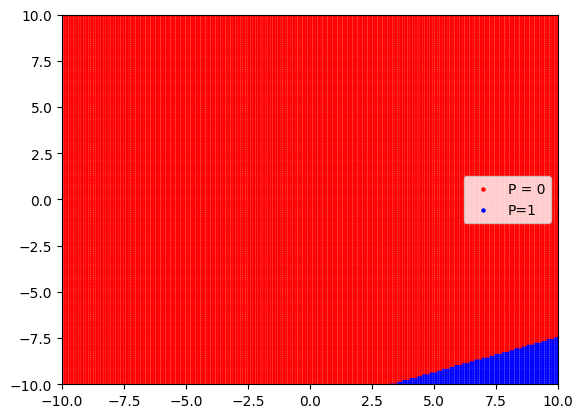
\includegraphics[width=\linewidth,height=0.8\paperheight,keepaspectratio=true]{linear_1.png}}
		\only<3>{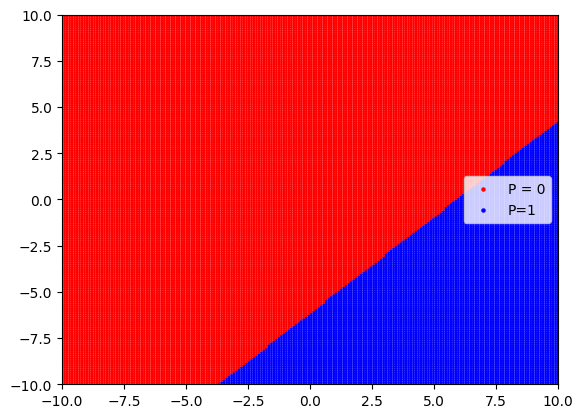
\includegraphics[width=\linewidth,height=0.8\paperheight,keepaspectratio=true]{linear_2.png}}
		\only<4>{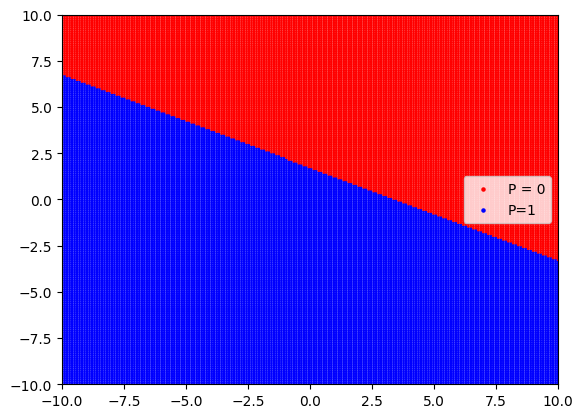
\includegraphics[width=\linewidth,height=0.8\paperheight,keepaspectratio=true]{linear_3.png}}
		\only<5>{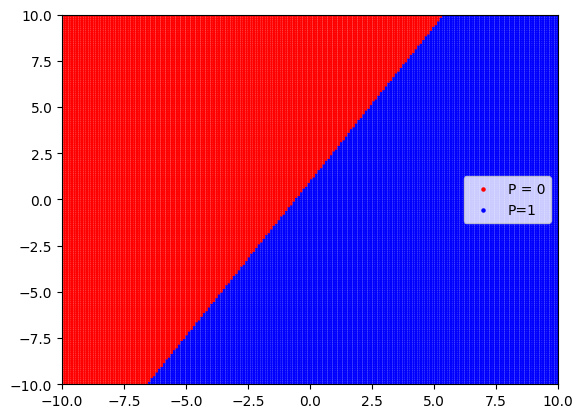
\includegraphics[width=\linewidth,height=0.8\paperheight,keepaspectratio=true]{linear_4.png}}
	\end{frame}

	{

	\nologo
	\begin{frame}{Affine Mess We Find Ourselves in}
		% Let's try chaining lots of pecreptrons together.....
		
		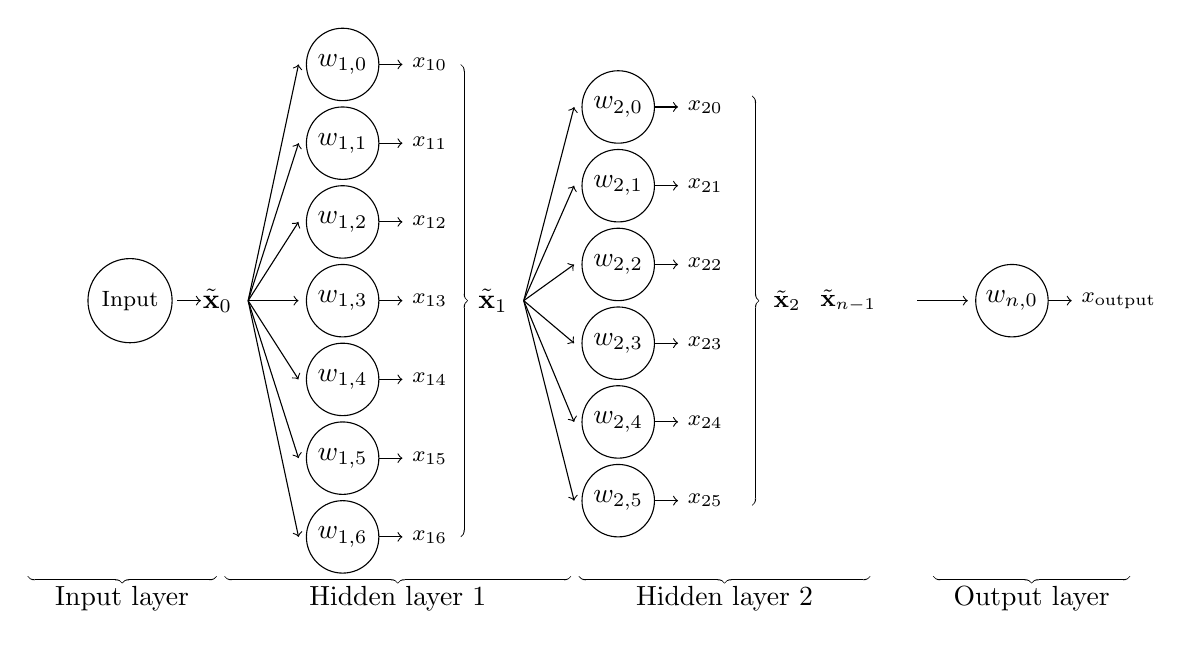
\begin{tikzpicture}
			% \draw (0,0) circle (0.4);
			\node[draw,circle] at (0.3,0) {\footnotesize Input};
			\draw[->] (0.9,0)--(1.2,0);
			\def\baseheight{-3.5}
			\draw [decorate, decoration = {calligraphic brace}] (1.4,\baseheight) --node[below]{Input layer}  (-1,\baseheight);
			\node[anchor=west] at (1.1,0) {$\tilde{\vec{x}}_0$};
			
			
			\foreach \i[count=\j from 0] in {3,2,...,-3}
			{
				\def\r{0.46}
				\def\y{\i}
				\def\x{3}
				\draw[->] (1.8,0)--({\x-\r-0.1},\y);
				\draw (\x,{\y}) circle ({\r});
				\node at (\x,{\y}) { $\cec{w}_{1,\j}$};
				\draw [->] ({\x+\r},{\y})--({\x+\r+0.3},{\y});
				\def\xx{\x+\r+0.3}
				% \draw[fill=white] ({\x-\r},{\y-\r})--({\x+\r},{\y-\r})--({\x+\r},{\y+\r})--({\x-\r},{\y+\r})--cycle;
				\node[anchor=west] at (\xx,{\y}) {\fontsize{8}{0}\selectfont$x_{1\j}$};%\phi_{1}^{\j}(y_{1}^{\j})$};
			}
			\draw [decorate, decoration = {calligraphic brace}] (4.5,3) --  (4.5,-3);
			\node[anchor=west] at (4.6,0) {$\tilde{\vec{x}}_1$};
			\draw [decorate, decoration = {calligraphic brace}] (5.9,\baseheight) --node[below]{Hidden layer 1}  (1.5,\baseheight);
			
			\foreach \i[count=\j from 0] in {2,1,0,-1,-2,-3}
			{
				\def\r{0.46}
				\def\y{\i+\r}
				\def\x{6.5}
				\draw[->] (5.3,0)--({\x-\r-0.1},\y);
				\draw (\x,{\y}) circle ({\r});
				\node at (\x,{\y}) { $\cec{w}_{2,\j}$};
				\draw [->] ({\x+\r},{\y})--({\x+\r+0.3},{\y});
				\def\xx{\x+\r+0.3}
				% \draw[fill=white] ({\x-\r},{\y-\r})--({\x+\r},{\y-\r})--({\x+\r},{\y+\r})--({\x-\r},{\y+\r})--cycle;
				\node[anchor=west] at (\xx,{\y}) {\fontsize{8}{0}\selectfont$x_{2\j}$};%\phi_{2}^{\j}(y_{2}^{\j})$};
			}
			\draw [decorate, decoration = {calligraphic brace}] (8.2,2.6) --  (8.2,-2.6);
			\draw [decorate, decoration = {calligraphic brace}] (9.7,\baseheight) --node[below]{Hidden layer 2}  (6,\baseheight);
			\node[anchor=west] (A) at (8.35,0) {\small$\tilde{\vec{x}}_2$};
			\node[anchor=west] at (A.east) {\small$\hdots\tilde{\vec{x}}_{n-1}$};
			\foreach \i[count=\j from 0] in {0}
			{
				\def\r{0.46}
				\def\y{\i}
				\def\x{11.5}
				\draw[->] (10.3,0)--({\x-\r-0.1},\y);
				\draw (\x,{\y}) circle ({\r});
				\node at (\x,{\y}) { $\cec{w}_{n,\j}$};
				\draw [->] ({\x+\r},{\y})--({\x+\r+0.3},{\y});
				\def\xx{\x+\r+0.3}
				% \draw[fill=white] ({\x-\r},{\y-\r})--({\x+\r},{\y-\r})--({\x+\r},{\y+\r})--({\x-\r},{\y+\r})--cycle;
				\node[anchor=west] at (\xx,{\y}) {\fontsize{8}{0}\selectfont${x}_\text{output}$};
			}
			
			\draw [decorate, decoration = {calligraphic brace}] (13,\baseheight) --node[below]{Output layer}  (10.5,\baseheight);
			% \draw [decorate, decoration = {calligraphic brace}] (15,1) --  (15,-1);
			% \node[anchor=west] at (15.2,0) {$\vec{x}_{n}$};
		\end{tikzpicture}
	\end{frame}

	\begin{frame}{Affine Mess We Find Ourselves in}
		% Let's try chaining lots of pecreptrons together.....
		
		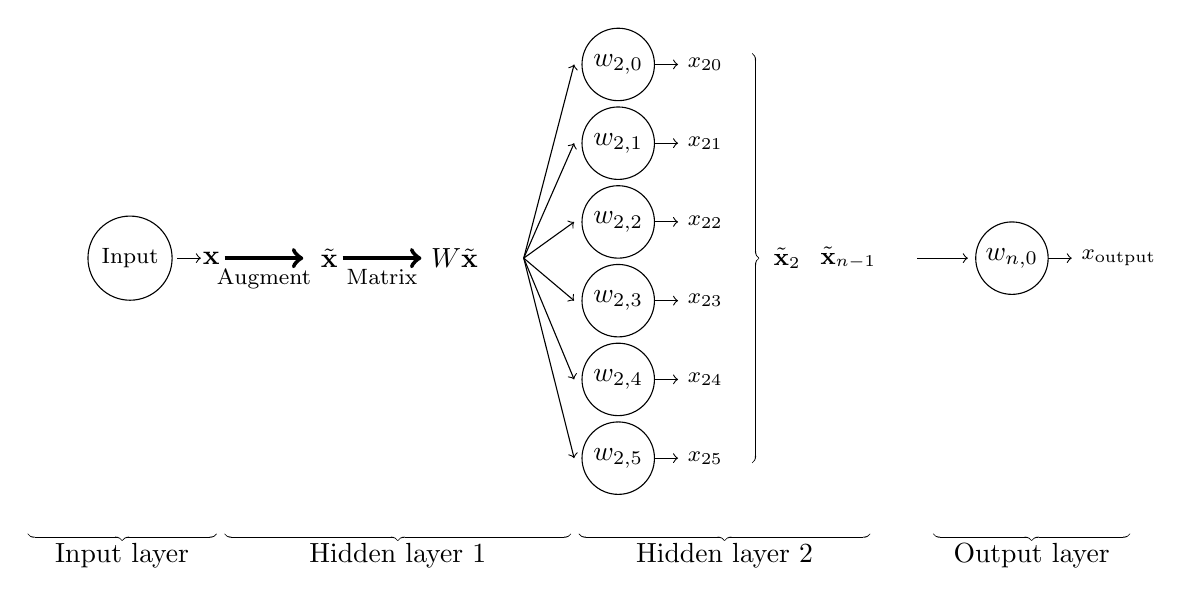
\begin{tikzpicture}
			% \draw (0,0) circle (0.4);
			\node[draw,circle] at (0.3,0) {\footnotesize Input};
			\draw[->] (0.9,0)--(1.2,0);
			\def\baseheight{-3.5}
			\draw [decorate, decoration = {calligraphic brace}] (1.4,\baseheight) --node[below]{Input layer}  (-1,\baseheight);
			\node[anchor=west] at (1.1,0) {${\vec{x}}$};

			\draw[ultra thick,->] (1.5,0)--node[below]{\footnotesize Augment}++(1,0);
			
			\node[anchor=west] at (2.6,0) {${\tilde{\vec{x}}}$};
			\draw[ultra thick,->] (3,0)--node[below]{\footnotesize Matrix}++(1,0);
	
			\node[anchor=west] at (4,0) {$ W \tilde{\vec{x}}$};
			\draw [decorate, decoration = {calligraphic brace}] (5.9,\baseheight) --node[below]{Hidden layer 1}  (1.5,\baseheight);
			
			\foreach \i[count=\j from 0] in {2,1,0,-1,-2,-3}
			{
				\def\r{0.46}
				\def\y{\i+\r}
				\def\x{6.5}
				\draw[->] (5.3,0)--({\x-\r-0.1},\y);
				\draw (\x,{\y}) circle ({\r});
				\node at (\x,{\y}) { $\cec{w}_{2,\j}$};
				\draw [->] ({\x+\r},{\y})--({\x+\r+0.3},{\y});
				\def\xx{\x+\r+0.3}
				% \draw[fill=white] ({\x-\r},{\y-\r})--({\x+\r},{\y-\r})--({\x+\r},{\y+\r})--({\x-\r},{\y+\r})--cycle;
				\node[anchor=west] at (\xx,{\y}) {\fontsize{8}{0}\selectfont$x_{2\j}$};%\phi_{2}^{\j}(y_{2}^{\j})$};
			}
			\draw [decorate, decoration = {calligraphic brace}] (8.2,2.6) --  (8.2,-2.6);
			\draw [decorate, decoration = {calligraphic brace}] (9.7,\baseheight) --node[below]{Hidden layer 2}  (6,\baseheight);
			\node[anchor=west] (A) at (8.35,0) {\small$\tilde{\vec{x}}_2$};
			\node[anchor=west] at (A.east) {\small$\hdots\tilde{\vec{x}}_{n-1}$};
			\foreach \i[count=\j from 0] in {0}
			{
				\def\r{0.46}
				\def\y{\i}
				\def\x{11.5}
				\draw[->] (10.3,0)--({\x-\r-0.1},\y);
				\draw (\x,{\y}) circle ({\r});
				\node at (\x,{\y}) { $\cec{w}_{n,\j}$};
				\draw [->] ({\x+\r},{\y})--({\x+\r+0.3},{\y});
				\def\xx{\x+\r+0.3}
				% \draw[fill=white] ({\x-\r},{\y-\r})--({\x+\r},{\y-\r})--({\x+\r},{\y+\r})--({\x-\r},{\y+\r})--cycle;
				\node[anchor=west] at (\xx,{\y}) {\fontsize{8}{0}\selectfont${x}_\text{output}$};
			}
			
			\draw [decorate, decoration = {calligraphic brace}] (13,\baseheight) --node[below]{Output layer}  (10.5,\baseheight);
			% \draw [decorate, decoration = {calligraphic brace}] (15,1) --  (15,-1);
			% \node[anchor=west] at (15.2,0) {$\vec{x}_{n}$};
		\end{tikzpicture}
	\end{frame}

	\begin{frame}{Affine Mess We Find Ourselves in}
		% Let's try chaining lots of pecreptrons together.....
		
		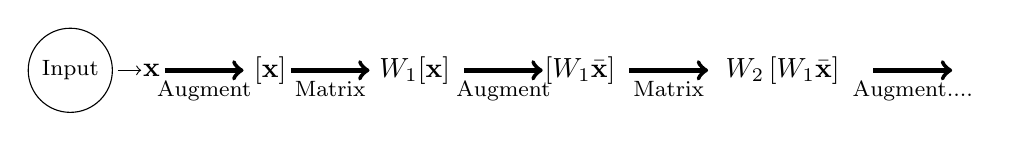
\begin{tikzpicture}
			% \draw (0,0) circle (0.4);
			\node[draw,circle] at (0.3,0) {\footnotesize Input};
			\draw[->] (0.9,0)--(1.2,0);
			\def\baseheight{-3.5}
			\node[anchor=west] at (1.1,0) {${\vec{x}}$};

			\draw[ultra thick,->] (1.5,0)--node[below]{\footnotesize Augment}++(1,0);
			
			\node[anchor=west] at (2.51,0) {${[{\vec{x}}]}$};
			\draw[ultra thick,->] (3.1,0)--node[below]{\footnotesize Matrix}++(1,0);
	
			\node[anchor=west] at (4.1,0) {$ W_1 [\vec{x}]$};

			\draw[ultra thick,->] (5.3,0)--node[below]{\footnotesize Augment}++(1,0);
			
			\node[anchor=west] at (6.2,0) {$\left[{{W_1\bar{\vec{x}}}}\right]$};
			\draw[ultra thick,->] (7.4,0)--node[below]{\footnotesize Matrix}++(1,0);
			\node[anchor=west] at (8.5,0) {$W_2\left[{{W_1\bar{\vec{x}}}}\right]$};
			
			\draw[ultra thick,->] (10.5,0)--node[below]{\footnotesize Augment....}++(1,0);

		
			% \draw [decorate, decoration = {calligraphic brace}] (15,1) --  (15,-1);
			% \node[anchor=west] at (15.2,0) {$\vec{x}_{n}$};
		\end{tikzpicture}
	\end{frame}

	}

	\begin{frame}{Affine Mess We Find Ourselves in}
		Or, in terms of \textbf{Affine Operators} (Chapter 3.4 in the notes):

		\vspace{0.5cm}

		$$\Bigg(\text{Affine = Matrix multiplicaiton + translation} \Longrightarrow \mathcal{W} \vec{v} = W \vec{v} + \vec{w} \Bigg)$$



		\vspace{0.5cm}
		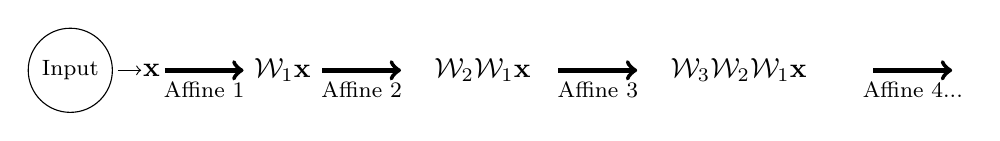
\begin{tikzpicture}
			% \draw (0,0) circle (0.4);
			\node[draw,circle] at (0.3,0) {\footnotesize Input};
			\draw[->] (0.9,0)--(1.2,0);
			\def\baseheight{-3.5}
			\node[anchor=west] at (1.1,0) {${\vec{x}}$};

			\pause\draw[ultra thick,->] (1.5,0)--node[below]{\footnotesize Affine 1}++(1,0);
			
			\node[anchor=west] at (2.51,0) {$\mathcal{W}_1 \vec{x}$};
			\pause\draw[ultra thick,->] (3.5,0)--node[below]{\footnotesize Affine 2}++(1,0);
	
			\node[anchor=west] at (4.8,0) {$ \mathcal{W}_2 \mathcal{W}_1 \vec{x}$};

			\pause\draw[ultra thick,->] (6.5,0)--node[below]{\footnotesize Affine 3}++(1,0);
			
			\node[anchor=west] at (7.8,0) {$\mathcal{W}_3 \mathcal{W}_2 \mathcal{W}_1 \vec{x}$};

			\draw[ultra thick,->] (10.5,0)--node[below]{\footnotesize Affine 4...}++(1,0);
			% \draw [decorate, decoration = {calligraphic brace}] (15,1) --  (15,-1);
			% \node[anchor=west] at (15.2,0) {$\vec{x}_{n}$};
		\end{tikzpicture}


		% \begin{spalign}
		% 	\vec{x}_1 & = \hat{\mathcal{W}_1} \vec{x}_\text{input}
		% 	\\
		% 	\vec{x}_2 & = \hat{\mathcal{W}_2} \vec{x}_1 = \hat{\mathcal{W}}_2 \hat{\mathcal{W}}_1 \vec{x}_\text{input}
		% 	\\
		% 	\vec{x}_3 & = \hat{\mathcal{W}_3} \vec{x}_2 =  \hat{\mathcal{W}}_3 \hat{\mathcal{W}}_2 \hat{\mathcal{W}}_1 \vec{x}_\text{input}
		% 	\\
		% 	\vdots
		% 	\\
		% 	x_\text{output} & = \begin{cases} 1 & \hat{\mathcal{W}_N} \vec{x}_{N-1} > 0 \\ 0 &\text{else} \end{cases}
		% \end{spalign}
	\end{frame}

	\begin{frame}{Affine Mess We Find Ourselves in}
		But...affine operators obey:
		\begin{equation}
			\hat{\mathcal{W}_2} \hat{\mathcal{W}_1} = \hat{\mathcal{V}}
		\end{equation}
		(Affine + Affine = Affine)

		Which means:

		\begin{equation}
			\hat{\mathcal{W}}_N \hat{\mathcal{W}}_{N-1} \hat{\mathcal{W}}_{N-2} \hdots \hat{\mathcal{W}}_{1}  \vec{x}_\text{input}  = \hat{\mathcal{V}} \vec{x}_\text{input} 
		\end{equation}

		\pause If you do the maths:

		\begin{equation}
			\hat{\mathcal{V}} \vec{x}= \vec{v} \cdot \vec{x} + \vec{b} 
		\end{equation}

		\pause Which is just....a single perceptron layer
	\end{frame}

	\begin{frame}{Affine Mess We Find Ourselves in}

		\begin{center}
			\bf If all you do is multiply by matrices \& add vectors, you will \textit{never} be doing anything other than an (extremely wasteful) perceptron algorithm
		\end{center}
		
	\end{frame}

	\begin{frame}{NonLinearity to the Rescue!}
		Need to break this affine relationship: enter \textbf{activation functions}.

	\end{frame}

	\begin{frame}{NonLinearity to the Rescue!}
	
		Let:
		\begin{equation}
			\vec{x}_n = \text{activate}\left(W \vec{x}_{n-1} + \vec{b} \right)
		\end{equation}
		
		\vspace{1cm}

		\pause One of the simples ways to break linearity is to add a \textit{elementwise function}:

		\begin{spalign}
			\vec{v} & = W \vec{x}_{n-1} + \vec{b}
			\\
			[\vec{x}_n]_i & = \sigma(v_i)
		\end{spalign}
		
	\end{frame}

	\begin{frame}{Elementwise Activation Functions}
		You can probably all name dozens of these functions in common use. 

		\begin{alignat*}{3}
			\text{Sigmoid /Logit}& \hspace{1cm} && \sigma(x) &&  = \frac{1}{1 + \exp(-x)} 
			\\
			\text{Rectified Linear Unit (ReLU)  } & &&\text{Relu}(x) && = \begin{cases} x & x > 0 \\ 0 &\text{else} \end{cases}
			\\
			\text{Leaky ReLU  } & && \text{Lelu}(x) && = \begin{cases} x & x > 0 \\ 0.01x &\text{else} \end{cases} 
			\\
			\text{tanh} & && \tanh(x) && = \frac{\exp(x) - \exp(-x)}{\exp(x) + \exp(-x)}
			\\
			\text{Softplus} & && \text{sft}(x) && = \log\left( 1+ \exp(x) \right)
		\end{alignat*}

		\textit{(Bonus Question: Can you name any commonly used functions which \textbf{don't} follow this pattern?)}
	\end{frame}


	\begin{frame}{NonLinearity Ahoy!}
	
		By replacing my (randomly initialised) hidden layers with Sigmoid nodes, I get:

		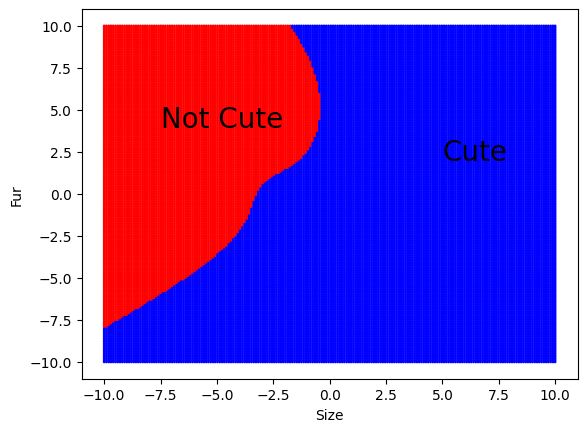
\includegraphics[width=\linewidth,height=0.8\paperheight,keepaspectratio=true]{NonLinearMLP.png}
	\end{frame}
\end{document}

